\documentclass[ExampleMasters.tex]{subfiles}

\tikzstyle{wide} = [rectangle, rounded corners, minimum width=1cm, minimum height=1cm,text centered, draw=black]
\tikzstyle{narrow} = [rectangle, rounded corners, minimum width=0.5cm, minimum height=1cm,text centered, draw=black]
\tikzstyle{narrow1} = [rectangle, rounded corners, minimum width=0.5cm, minimum height=1cm,text width = 3cm, text centered, draw=black]
\tikzstyle{arrow} = [thick,->,>=stealth]

\begin{document}

\chapter{Mission Productivity}

	\section{Introduction}
		The addition of electric propulsion on axles other than the conventional engine-propelled axles in long combinations is necessary to meet power and gradeability requirements as well as the performance based standards. The choice of axles is to be well-motivated and quantifiable. An objective numerical standard of comparison between different combinations and propulsion configurations for specific missions can thus be provided by the mission productivity factor. The objective function used to represent mission productivity will be sought to be maximised. In the following sections, various definitions of mission productivity in the heavy truck transport context will be presented. The definition chosen to be optimised will then be formulated and discussed in detail.\\ 

	\section{Mission productivity definitions}
		Productivity is expressed as the number of units of output that a given number of units of input / investment yields. OECD defines productivity as "the ratio of a volume measure of output to a volume measure of input"\cite{OECDProd}. The outputs of a production or transport process are often influenced by a combination of several factors or 'inputs', that may themselves be dependent on one another. Depending on the nature and quantity of reference inputs against which productivity is measured, the latter can be classified as follows \cite{JapSNAOECD}:

		\begin{itemize}
			\item \textbf{Single factor productivity} - The outputs of a process are often measured relative to a single input either due to its relative importance among all possible factors or to observe the individual trends of output performance specific to the input chosen. For example, labour or workforce productivity measures the volume output relative to the number of working hours spent by an employee \cite{TruckProdAus, WikiLabourProd}. In the current perspective, the mission productivity relative to a single factor such as driver expenses or fuel consumption is an example of such a measure.

			\item \textbf{Multi-factor productivity} - When the influences of several individual inputs to a system or process are considered inseperable, the productivity measure is defined relative to a combination of all the inputs expressed suitably as an expression. For example, the Gross Domestic Product is a productivity measure relative to a host of factors such as population, economy and education among several others \cite{TruckProdAus, WikiGDP}. In the current context, mission productivity can be expressed with respect to a combination of factors such as fuel economy, electricity prices, driver costs, maintenance costs and fixed purchasing costs. 
		\end{itemize}

		The productivity measure for a heavy truck-trailer combination serves as a fitness measure to evaluate the economic and environmental viability of the combination on a given specific mission. It can be deduced from the above that the fitness measure is hence mission dependent and is thus bound to vary depending on the route chosen, type of payload carried, number of starts and stops and driver behaviour among several other mission parameters. Thus, it can inferred that the productivity measure, when optimised for each mission, will yield different optimal combinations suited for the mission at hand.\\

		A few different mission productivity measures are briefly considered below:
		\begin{itemize}
			\item \textit{Load per vehicle kilometre} - This single factor productivity measure, P1, focuses on the quantity of payload transported for every kilometre of vehicle distance covered and can thus be optimised by reducing mission time to increase number of annual trips, increase axle load capacities and improving average combination speeds while preserving key performance characteristics such as gradeability. These can be achieved by employing an improved powertrain or increased axle propulsion. The measure does not consider fuel consumption, fixed costs etc. though.

			\begin{equation}
				P1 = \frac{M_{payload} \times N_{trips}}{D_{annual}} \ tons/km
			\end{equation}

			where $N_{trips}$ is the average annual number of trips covered for the given mission, $M_{payload}$ is the average load carried per mission (kg) and $D_{annual}$ is the average total vehicle distance covered (km).

			\item \textit{Annual freight per vehicle} - This measure, P2, is indicative of the utilisation of the vehicle and is expressed in number of tonne-kilometres covered annually \cite{TruckProdAus}. Thus, the number of useful transportation kilometres coupled with the quantity of payload transported forms the basis for the measure. This too, does not consider fuel consumption and other mission outputs.

			\begin{equation}
				P2 = M_{payload} \times D_{annual} \ tonne-km
			\end{equation}

			\item \textit{Average operating costs per vehicle kilometre or freight transported} - The operating costs involve fuel consumption, driver expenses and maintenance costs and are sought to be minimised against every unit tonne-kilometre freight. While this measure, P3, is a more meaningful quantity, it fails to adequately address the business profitability of ownership and transport.

			\begin{equation}
				P3 = \frac{Cost_{operating}}{M_{payload} \times D_{annual}},\ or\ \frac{Cost_{operating}}{D_{annual}} \  \euro/tonne-km \ or \ \euro/km 
			\end{equation}

			where $Cost_{operating}$ is the average annual operating cost. This may itself be expressed as 

			\begin{equation}
				Cost_{operating} = Cost_{fuel} + Cost_{personnel} + Cost_{maintenance} + Cost_{miscellaneous} \ \euro
			\end{equation}

			where $Cost_{fuel}$ is the average annual fuel expense, $Cost_{personnel}$ is the average annual cost incurred by employment of personnel including the driver, $Cost_{maintenance}$  is the average annual cost of maintenance of the truck and associated operational elements and $Cost_{miscellaneous}$ is the sum of all miscellaneous costs arising from the freight transport.\\

			\item \textit{Freight per driver hour} - In developed economies, personnel costs in heavy trucking can account for upto 44\% in long haul operations. The dominant contribution of personnel expenses to transportation costs thus implies that the freight transport productivity relative to investment in drivers and other personnel, P4, must be maximised. This, of course, must not be achieved at the expense of high fuel prices resulting from aggressive driving to minimise mission times. 

			\begin{equation}
				P4 = \frac{M_{payload} \times D_{annual}}{T_{driver}} \ tonne-km/hour
			\end{equation}

			where $T_{driver}$ is the average annual number of driver hours billed to the freight transport company (including rest and halt hours).\\

			\item \textit{Freight per unit fuel consumed} - The ratio of driver to fuel expenses is reversed in developing economies where fuel prices can account for upto 45\% of the transportation costs. Here, maximising the freight transport per litre of fuel consumed, P5, becomes more pertinent.
			
			\begin{equation}
				P5 = \frac{M_{payload} \times D_{annual}}{V_{fuel}} \ tonne-km/litre
			\end{equation}

			where $V_{fuel}$ is the average annual fuel consumption in litres.\\

			\item \textit{Emissions per unit freight transported} - The environmental impact of freight transport can be quantified in terms of the number of milligrams of carbon dioxide emissions generated per tonne-kilometre of freight transported, P6. This become relevant especially in the current context where additional electric propulsion can improve not only vehicle gradeability and average speed, but also reduce vehicle emissions. The combination that has the least carbon footprint for the given mission can thus be identified and the transportation expenses viewed more holistically. The fixed costs in the optimisation schedule will thus vary depending on the exhaust after-treatment systems used; maintenance costs will depend on the quantity of AdBlue used, number of diesel particulate filters replaced etc.

			\begin{equation}
				P6 = \frac{M_{emissions}}{M_{payload} \times D_{annual}}\  mg/tonne-km
			\end{equation}

			where $M_{emissions}$ is the average annual number of milligrams of carbon dioxide and other noxious pollutant emissions generated by the vehicle.

			\item \textit{Revenue earned per unit investment} - From the logistics provider's perspective, the maximisation of returns on investment, or profit maximisation, over a fixed number of years is primal. This depends not only on the freight transported, driver, fuel and maintenance expenses and fixed initial costs, but also on the type of payload being transported and the revenue earned from each mission. This measure, P7, is thus a multi-factor productivity factor that is sensitive to several input factors as mentioned above.

			\begin{equation}
				P7 = \frac{Revenue_{annual} \times N_{first\ owner}}{Cost_{fixed} + Cost_{variable}}\ \euro/\euro
			\end{equation}

			where $Revenue_{annual}$ is the average annual revenue earned over a target duration of $N_{first\ owner}$ years, $Cost_{fixed}$ is the initial investment in the tractor, trailers and machinery and $Cost_{variable}$ is the total operating cost over $N_{first\ owner}$ years.

		\end{itemize}

		While single factor productivity measures such as fuel costs per kilometre travelled are valid figures, their relevance can be skewed when viewed in a wider perspective. For example, as shown in Table \ref{table:fuelConsumptionRate} \cite[T.~2.8]{TruckProdAus}, the average fuel consumption per kilometre travelled for articulated trucks increased from 45.7 to 49.5 litres per 100 kilometres during the years 1971 and 2007. During the same period of time, in comparison, the fuel consumption per unit freight (tonne-kilometre) dropped by 44\% from 4.7 to 2.7 litres per 100 ton-kilometres \cite{TruckProdAus}. Hence, the choice of productivity measure is key to arriving at the right objective function to optimise.\\

		\begin{table}[ht]
			\centering 
			\begin{tabular}{l c c c c}
  			\hline
			Vehicle type & \multicolumn{4}{c}{Fuel consumption rate}\\ \cline{2-3} \cline{4-5}
			\ & \multicolumn{2}{c}{Per VKT} & \multicolumn{2}{c}{Per TKM}\\ \cline{2-3} \cline{4-5}
			\ & 1971 & 2007 & 1971 & 2007\\ \hline
			    LCVs  & 12.8 & 12.8 & 108.7 & 60.7\\
			    Rigid trucks  & 23.3 & 26.0 & 12.7  & 7.2\\
			    Articulated trucks  & 45.7 & 49.5 & 4.7 & 2.7  \\
			    All CVs  & 27.9 & 36.4 & 8.1 & 3.5 \\
			    All HVs  & 19.9 & 19.8 & 11.8 & 6.2 \\
			\hline 
			\end{tabular}
			\caption{Fuel consumption per freight tonne kilometre, 1971-2007 \cite{TruckProdAus}} 
			\label{table:fuelConsumptionRate} 
		\end{table}

		Since profit maximisation of transport customers is the object of prime focus while choosing freight transport configurations, it can be agreed that the corresponding productivity measure is a multi-factor one, depending on a number of input parameters as explained in the forthcoming section.\\

	\section{Productivity measure - Choice and Description}

		The goals sought to be achieved by the European Modular Systems as set out by the EMS Internal Platform Group are as follows \cite{EMSleaflet}:
		\begin{itemize}
			\item Meeting growing freight transport demands
			\item Reducing fuel consumption
			\item Reducing emissions
			\item Reducing operating costs for freight transporters
		\end{itemize}

		\begin{figure}[h!]
			\centering
			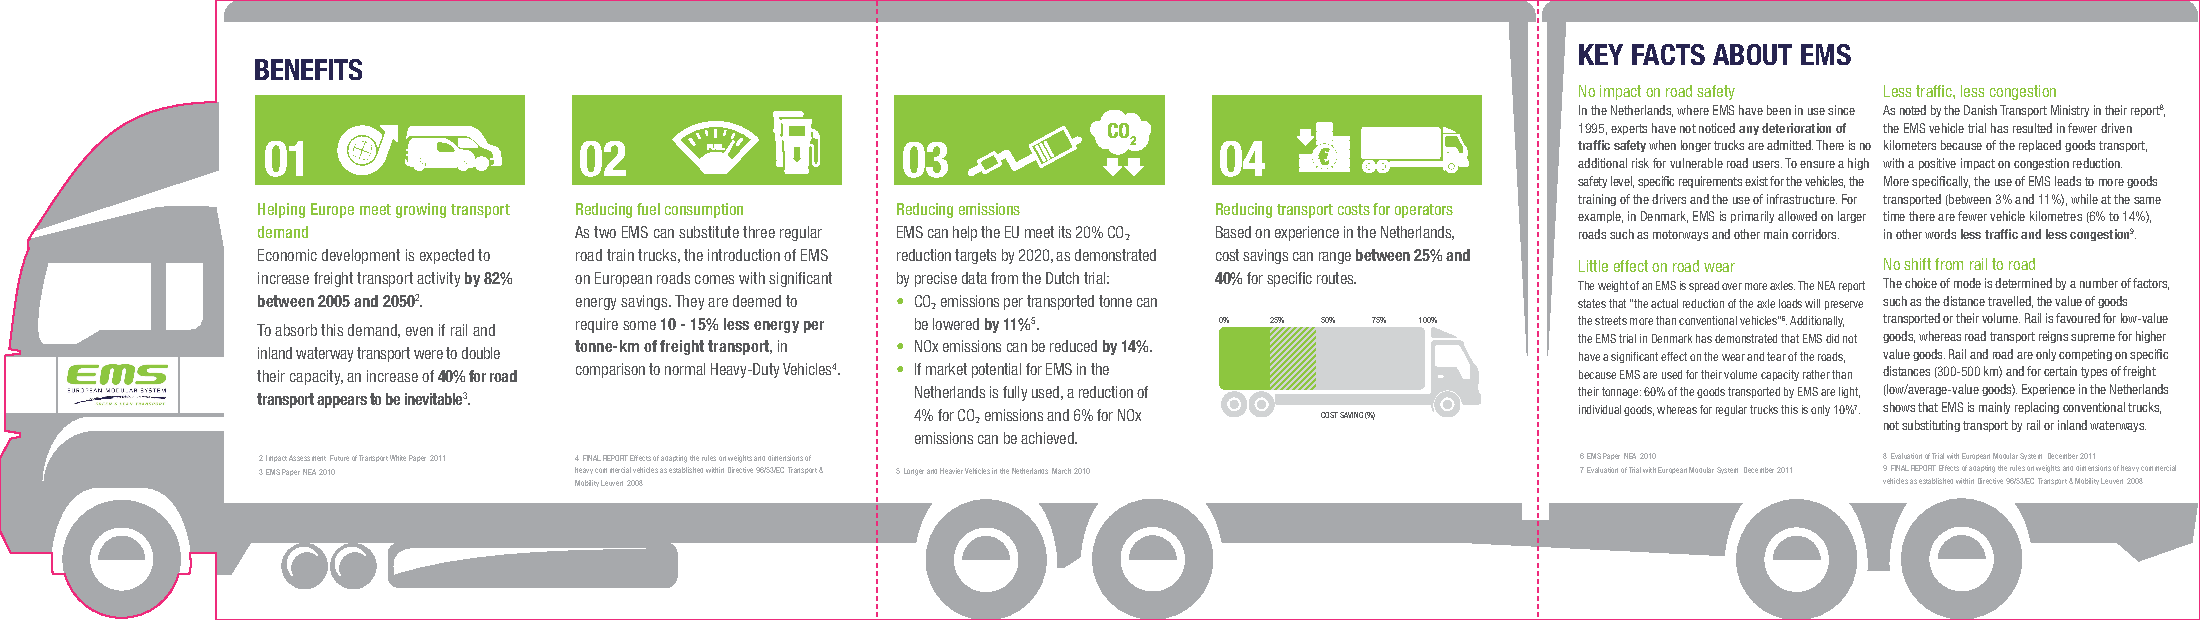
\includegraphics[width=\linewidth, clip=true, trim=0 0 325 0]{figures/eea_leaflet.pdf}
			\caption{Goals of the European Modular System \cite{EMSleaflet}}
			\label{EMSleaflet}
		\end{figure}

		It can hence been seen that, seen from the freight transporter's prespective, the productivity measure must focus on maximising freight carried while capping fuel consumption and associated emissions, while still producing revenues that promote profit maximisation. Thus, the last productivity measure defined in the previous section, revenue earned per unit investment, is chosen as a reasonable complete measure that incorporates the salient goals of the EMS.\\ 

		The productivity factor, P, is redefined below for clarity:
		\begin{equation} \label{eq:productivity}
			P = \frac{Revenue_{annual} \times N_{first\ owner}}{Cost_{fixed} + Cost_{variable}}\ \euro/\euro
		\end{equation}

		where $Revenue_{annual}$ is the average annual revenue earned over a target duration of $N_{first\ owner}$ years, $Cost_{fixed}$ is the initial investment in the tractor, trailers and machinery and $Cost_{variable}$ is the total operating cost over $N_{first\ owner}$ years.\\

		$Revenue_{annual}$ is usually defined in terms of the average gross transporter income or gross transport costs per unit freight transported, per vehicle kilometer. It can be gleaned from literature that the former definition is known to vary between 4 and 6 US Dollar Cents per tonne-kilometre \cite{WorldBankReport} while the latter is in the range of 0.75 USD per kilometre to 1.25 USD per kilometre \cite{WorldBankReport}.\\

		The initial buying prices of trucks, trailers, additional loading equipment and superstructures form the bulk of the fixed costs, $Cost_{fixed}$. Average truck prices in the context of the European buyer are considered in this thesis, with a step-up margin for the three different powertrain sizes considered in the optimisation tool. It must be noted though, that the axle load configurations, cab specifications and other truck parameters have a significant bearing on actual buying prices, aside from taxation policies and registration schedules that vary internationally. Frost \& Sullivan \cite{FrostSullivan} estimates average upfront truck prices ranging between 105,000 USD and 130,000 USD and trailer prices ranging between 40,000 USD and 70,000 USD for the year 2014. This thesis places the dolly and semitrailer prices at the lower and upper bounds for the trailer prices respectively. The truck price is assigned to the base powertrain configuration and premiums of x\% and y\% are assigned to the higher powertrain configurations respectively, based on Volvo's Cost-Calc tool.\\

		In this thesis, the price of electrified axles is incorporated in the form of add-on features and are thus simple additive terms to the base price of the trailer. The electrification charges are divided primarily among the batteries, the electric machine and the auxiliary power electronics and control systems. Additionally, the additional mass of the electrification components is penalised by an appropriate reduction in payload tonnage capacity. Advances in battery technology are rapid and are expected to yield significant cost advantages over the years. Hence, a price trend analysis is necessary to evaluate how mission productivities can be maximised by the availability of cheaper batteries with higher energy densities in the decades to come. Lithium-ion batteries for plug-in hybrid vehicles with energy capacities in the range of 15-21 kWh are priced between 800 and 1200 \euro per kilowatt-hour today \cite{EUROBAT} and are expected to fall to 450 \euro per kilowatt-hour in the next decade \cite{EUROBAT}. The long-term trends predicted and published in \cite[T.~8-16]{ElementEnergy} are referenced for evaluations in productivity sensitivity to battery prices and are as shown in Table \ref{table:batteryPriceMassTrend}.\\

		\begin{table}[ht]
			\centering 
			\begin{tabular}{l c c c c c}
				\cline{2-6}
				\ & 2011 & 2015 & 2020 & 2025 & 2030\\ 
				\hline
			    Pack cost (USD/kWh)  & 746 & 436 & 275 & 244 & 230\\
			    Pack mass (kg)  & 343 & 253 & 195  & 177 & 176\\
				\hline 
			\end{tabular}
			\caption{Battery price and mass trends 2011-2030 \cite{ElementEnergy}} 
			\label{table:batteryPriceMassTrend} 
		\end{table}

		DC electric motors rated between 75kW and 350kW are found to be priced approximately 29900 EUR \cite{EuPLot30Motors}.

		Variable costs or operational costs were estimated at approximately 80 \euro / hour for France and Germany \cite{EuAECOM1} with driver costs amounting to upto 38\% of the total operating costs. The contributors to total operating costs were referenced from the European Commission study \cite[T.~7b]{EuAECOM2} and average values tabulated below in Table \ref{table:OperatingCostContributors}.\\

		\begin{table}[ht]
			\centering 
			\begin{tabular}{l c}
				\hline
				\ & Percentage contribution (\%)\\
				\hline
			    Driver  & 35\\
			    Fuel  & 22\\
			    Insurances, tolls and taxes & 14\\
			    Tyres & 7\\
			    Maintenance & 6\\
				\hline 
			\end{tabular}
			\caption{Contributors to total operating costs \cite[T.~7b]{EuAECOM2}} 
			\label{table:OperatingCostContributors} 
		\end{table}

		Average driver hourly wages varied between 12 and 24 \euro / hour in the EU \cite[T.~7.2]{EuAECOM1}. The average diesel price for the 27-member EU was 1.468 \euro / litre in April 2013 \cite[T.~7.3]{EuAECOM1}. Fuel price is considered to evolve at 3\% each year \cite[C.~14]{LongHaulFH}. The average price of electricity that will be used to recharge batteries in plug-in hybrid vehicles is 0.21 \euro / kWh \cite{EUelectricity}. Electricity price evolution is also fixed at 3\% per year \cite[T.~14]{LongHaulFH}. Armed with these figures, a mathematical formulation for the productivity can be derived and a sensitivity analysis performed.  

	\section{Productivity formulation}

		The productivity formulation is now developed mathematically. As can be deduced, the mission productivity is desired to be as large as possible. The mission reveneues, fixed costs and operating costs are dealt with in succession.

		\begin{equation} \label{eq:productivity}
			P = \frac{R_N}{C_{fixed} + C_{variable,\ N}}\ \euro/\euro
		\end{equation}

		\subsection{Mission revenues}

		The average revenue earned per unit freight carried, $R_{unit\ freight}$ \euro \ has been discussed in the earlier section and is used to arrive at annual mission revenues.

		\begin{equation}
			R_{mission} = R_{unit\ freight} \times M_{payload,\ net} \times D_{mission} \  \euro / mission
		\end{equation}
		where, $R_{mission}$ is the revenue earned per mission (\euro). The net payload carried $M_{payload,\ net}$ is expressed as:

		\begin{equation}
			M_{payload,\ net} = M_{payload,\ gross} - \Delta M_{eAxle}
		\end{equation}
		where the total mass due to propulsion of additional axles on trailers is $\Delta M_{eAxle}$ \ \euro \ and $M_{payload,\ gross}$ is the mass of the payload carried by the conventional combination. 

		\begin{equation}
			R_{annual} = R_{mission} \times N_{mission,\ annual} \  \euro / year
		\end{equation}
		where, $N_{mission,\ annual}$ is the average annual number of trips made and $R_{annual}$ is the total annual mission revenue earned by the freight transporter (\euro). \\

		The level of utilisation of the available axle load capacity and trailer volume is represented using a vehicle utilisation factor $U$. The combination is certified volume or tonnage limited based on if $V_{payload,\ max} \times \rho_{payload} \leq M_{axle, max}$. The utilisation factor is then defined as below:

		\begin{equation}
			U = \frac{M_{payload,\ gross}}{M_{axle,max}}\ (Tonnage-limited)
		\end{equation}
		or,

		\begin{equation}
			U = \frac{V_{payload,\ gross}}{V_{payload,\ max}}\ (Volume-limited)
		\end{equation}

		This can thus be used as an adjustment factor to express annual mission revenues, when employed in a comparitive sense, like in the case of optimisation.

		\begin{equation}
			R_{annual,\ corrected} = R_{annual} \times \frac{1}{U}
		\end{equation}

		The revenue earned over the target first owner duration of $N_{first\ owner}$ years is then calculated as:

		\begin{equation}
			R_{N} = R_{annual,\ corrected} \times N_{first\ owner} \  \euro
		\end{equation}

		\subsection{Fixed costs}

			The total fixed costs of the combination are expressed as a sum of the conventional combination and the cost incurred in addition of propulsion on trailer axles on successive units.

			\begin{equation}
				C_{fixed} = C_{fixed,\ conv}+ \displaystyle \sum_{i=2}^{N_{units}} C_{fixed,\ elec, i}
			\end{equation}
			where,

			\begin{equation}
				C_{fixed,\ conv} = P_{tractor,\ net}+P_{dolly}+P_{ST,1}+P_{ST,2}
			\end{equation}
			Premiums on higher powertrains $\Delta P_{powertrain}$ are added as:
			
			\begin{equation}
				P_{tractor,\ net} = P_{tractor,\ base} + \Delta P_{powertrain}
			\end{equation}
			where $P_{tractor,\ base}$ is the price of the tractor with the base powertrain configuration. 

			\begin{equation}
				C_{fixed,\ elec, i} = P_{batt,i}+\displaystyle \sum_{j=1}^{N_{eAxle,i}} P_{eAxle,j}
			\end{equation}
			The battery price for a single unit i, $P_{batt,i}$, is expressed as
			\begin{equation}
				P_{batt,i}= S_{batt} \times P_{batt/kWh}
			\end{equation}
			The price of the electrically propelled axle $P_{eAxle,j}$ consists of the electric machine, power electronics and transmission components, all of which are considered to be included in the electric motor prices discussed in the previous section. The total mass of electric axles, represented by $\Delta M_{eAxle}$ in the previous subsection can be expressed as:

			\begin{equation}
				\Delta M_{eAxle} = \displaystyle \sum_{i=2}^{N_{units}} M_{eAxle,i}
			\end{equation}
			where, 
			\begin{equation}
				M_{eAxle,i} = (M_{battery,i} - \sum_{j=1}^{N_{eAxle,i}} M_{mot,j}) \forall i=2,..N_{units}
			\end{equation}

		\subsection{Operational Costs}
			The total mission variable operational costs $C_{variable}$ are expressed
			
			\begin{equation}
				C_{variable,\ mission} = C_{driver} + C_{fuel} + C_{mnt} + C_{tyres} + C_{tolls} + C_{elec}
			\end{equation}

			\begin{equation}
				C_{driver} = T_{mission} \times C_{driver, hour}
			\end{equation}
			where driver hourly wages $C_{driver, hour}$ are as discussed in the previous section.

			\begin{equation}
				C_{fuel} = V_{fuel} \times C_{fuel, litre}
			\end{equation}
			where the fuel costs $C_{fuel, litre}$ are the average EU-27 costs mentioned earlier. Maintenance costs $C_{mnt}$ are expressed in terms of a relative ratio to driver costs, $R_{mnt-driver}$. Ratios are as derived from Table \ref{table:OperatingCostContributors}.

			\begin{equation}
				C_{mnt} = C_{driver} \times R_{mnt-driver}
			\end{equation}
			Tyre maintenance costs and tolls are also expressed in a similar fashion as below:

			\begin{equation}
				C_{tyres} = C_{driver} \times R_{tyre-driver}
			\end{equation}

			\begin{equation}
				C_{tolls} = C_{driver} \times R_{toll-driver}
			\end{equation}
			The electricity charges incurred on recharging buffers in case of the plug-in hybrid are expressed as:

			\begin{equation}
				C_{elec} = E_{recharge} \times P_{elec/kWh}
			\end{equation}
			The annual operational costs are extended over the $N_{first\ owner}$ years to arrive at total operation costs:

			\begin{equation}
				C_{variable,\ N} = C_{variable,\ mission} \times N_{first\ owner} \times N_{mission,\ annual}
			\end{equation}


\end{document}